%!TEX root = ../main.tex
\setchapterimage[7.5cm]{figs/fundamentales/pilares}
\setchapterpreamble[u]{\margintoc}

\chapter{Conceptos fundamentales} \label{chap:fundamentales}

\begin{kaobox}
	``El placer más noble es el júbilo de comprender"
	\begin{flushright}
		Leonardo da Vinci
	\end{flushright}
\end{kaobox}


Se inicia mostrando las hipótesis básicas adoptadas en la estática de estructuras.


\section{Esfuerzos}
	
	\subsection{Tensor esfuerzo de Cauchy}
	\index{Tensor de esfuerzo} \index{Cauchy}
	Un punto $P$ cualquiera de un cuerpo bajo la acción de fuerzas
	externas o internas\sidenote[][3cm]{Las fuerzas internas se conocen como fuerzas de cuerpo.} está sometido a unos esfuerzos reunidos en el \textit{tensor de esfuerzos Cauchy}\sidenote[][3.5cm]{Augustin-Louis Cauchy, francés (21 Agosto 1789 – 23 Mayo 1857)} (ver fig. \ref{Sigmas}).
	
	\begin{figure}[ht]
		\centering
		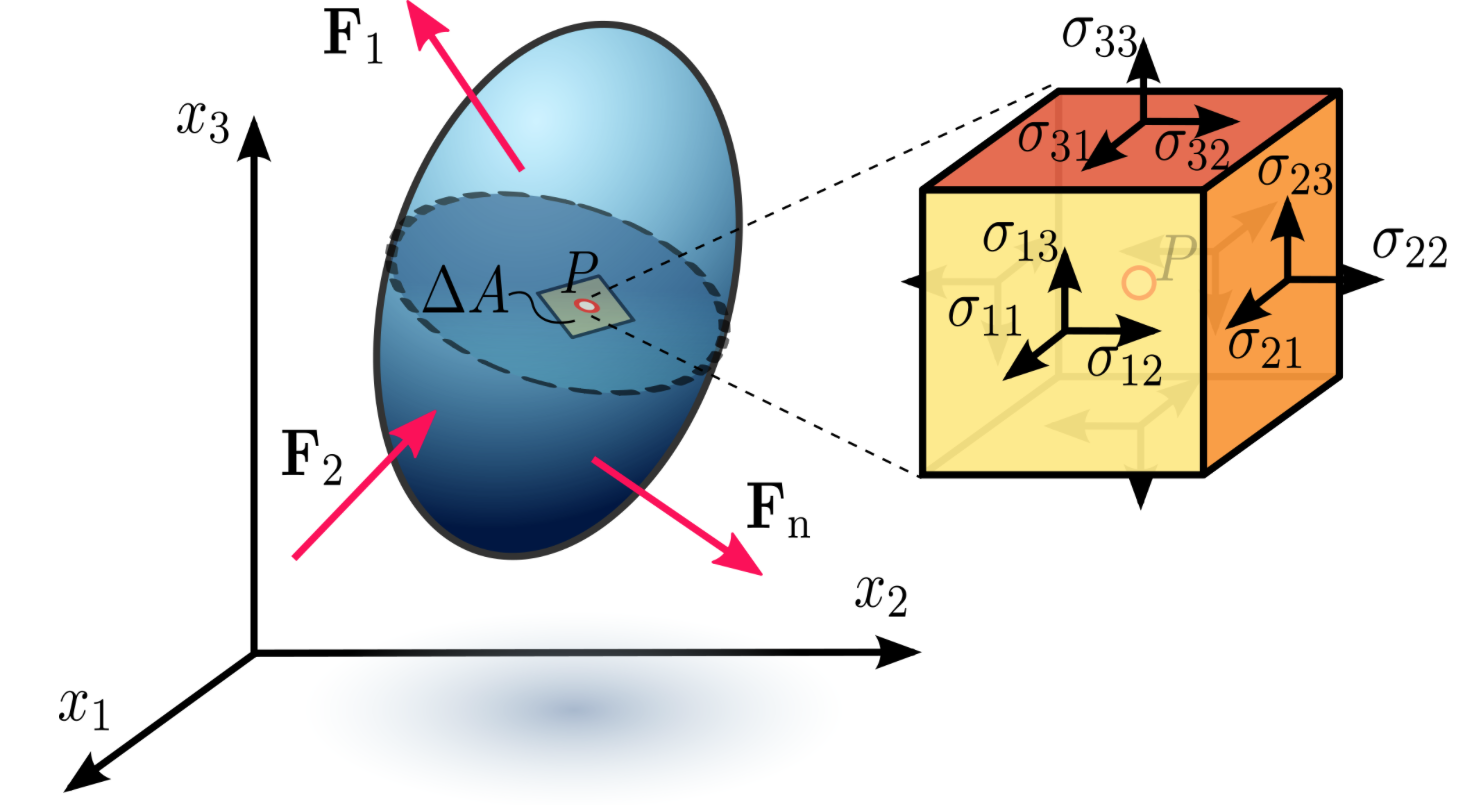
\includegraphics[width=0.75\textwidth]{figs/intro/Sigmas}
		\caption{Esfuerzos en un punto}
		\label{Sigmas}
	\end{figure}
	
	\begin{equation}
		\bm{\sigma} \coloneqq \begin{bmatrix}
			\sigma_{11} & \sigma_{12} & \sigma_{13} \\
			\sigma_{21} & \sigma_{22} & \sigma_{23} \\
			\sigma_{31} & \sigma_{32} & \sigma_{33}
		\end{bmatrix} = \begin{bmatrix}
			\sigma_x & \tau_{xy} & \tau_{xz} \\
			\tau_{yx} & \sigma_y & \tau_{yz} \\
			\tau_{zx} & \tau_{zy} & \sigma_z
		\end{bmatrix}
		\label{CauchyTensor}
	\end{equation}
\marginnote[-1.2cm]{\small Tensor de esfuerzos de Cauchy}
	
	Se utiliza la correspondencia siguiente:
	\begin{equation*}
		\begin{array}{ccc}
			x_1 \rightarrow x; & x_2 \rightarrow y; & x_3 \rightarrow z
		\end{array}
	\end{equation*}
	
	El tensor de esfuerzos de Cauchy es simétrico, esta simetría permite escribirlo en formato vectorial:
	\begin{equation}
	    \underline{\bm{\sigma}} = \begin{bmatrix} \sigma_x & \sigma_y & \sigma_z & \tau_{yz} & \tau_{xz} & \tau_{zy} \end{bmatrix}^T
	\end{equation}
	
	aplicado a pórticos planos se reduce a:
	\begin{equation}
	    \underline{\bm{\sigma}} = \begin{bmatrix} \sigma_{x} & \sigma_{y} & \tau_{xy} \end{bmatrix}
	\end{equation}
	
	en problemas unidimensionales:
	\begin{equation}
	    \underline{\bm{\sigma}} = \sigma_x
	\end{equation}

En general, para un problema tridimensional $\bm{\sigma} \in \mathbb{R}^6$, en el caso bidimensional $\bm{\sigma} \in \mathbb{R}^3$ y, en problemas unidimensionales $\bm{\sigma} \in \mathbb{R}$.

\subsection{Vector de tracción de Cauchy}
	
	\index{Vector de tracción de Cauchy}
	Observando ahora la fig. \ref{fig:TetraCauchy} y la fig. \ref{Sigmas} anterior, se puede demostrar sin dificultad la siguiente relación entre \textit{vector de tracción de Cauchy} $\mathbf{T}$ y  el \textit{tensor de esfuerzos de Cauchy} $\bm{\sigma}$:
	
	\marginpar{
\captionsetup{type=figure}
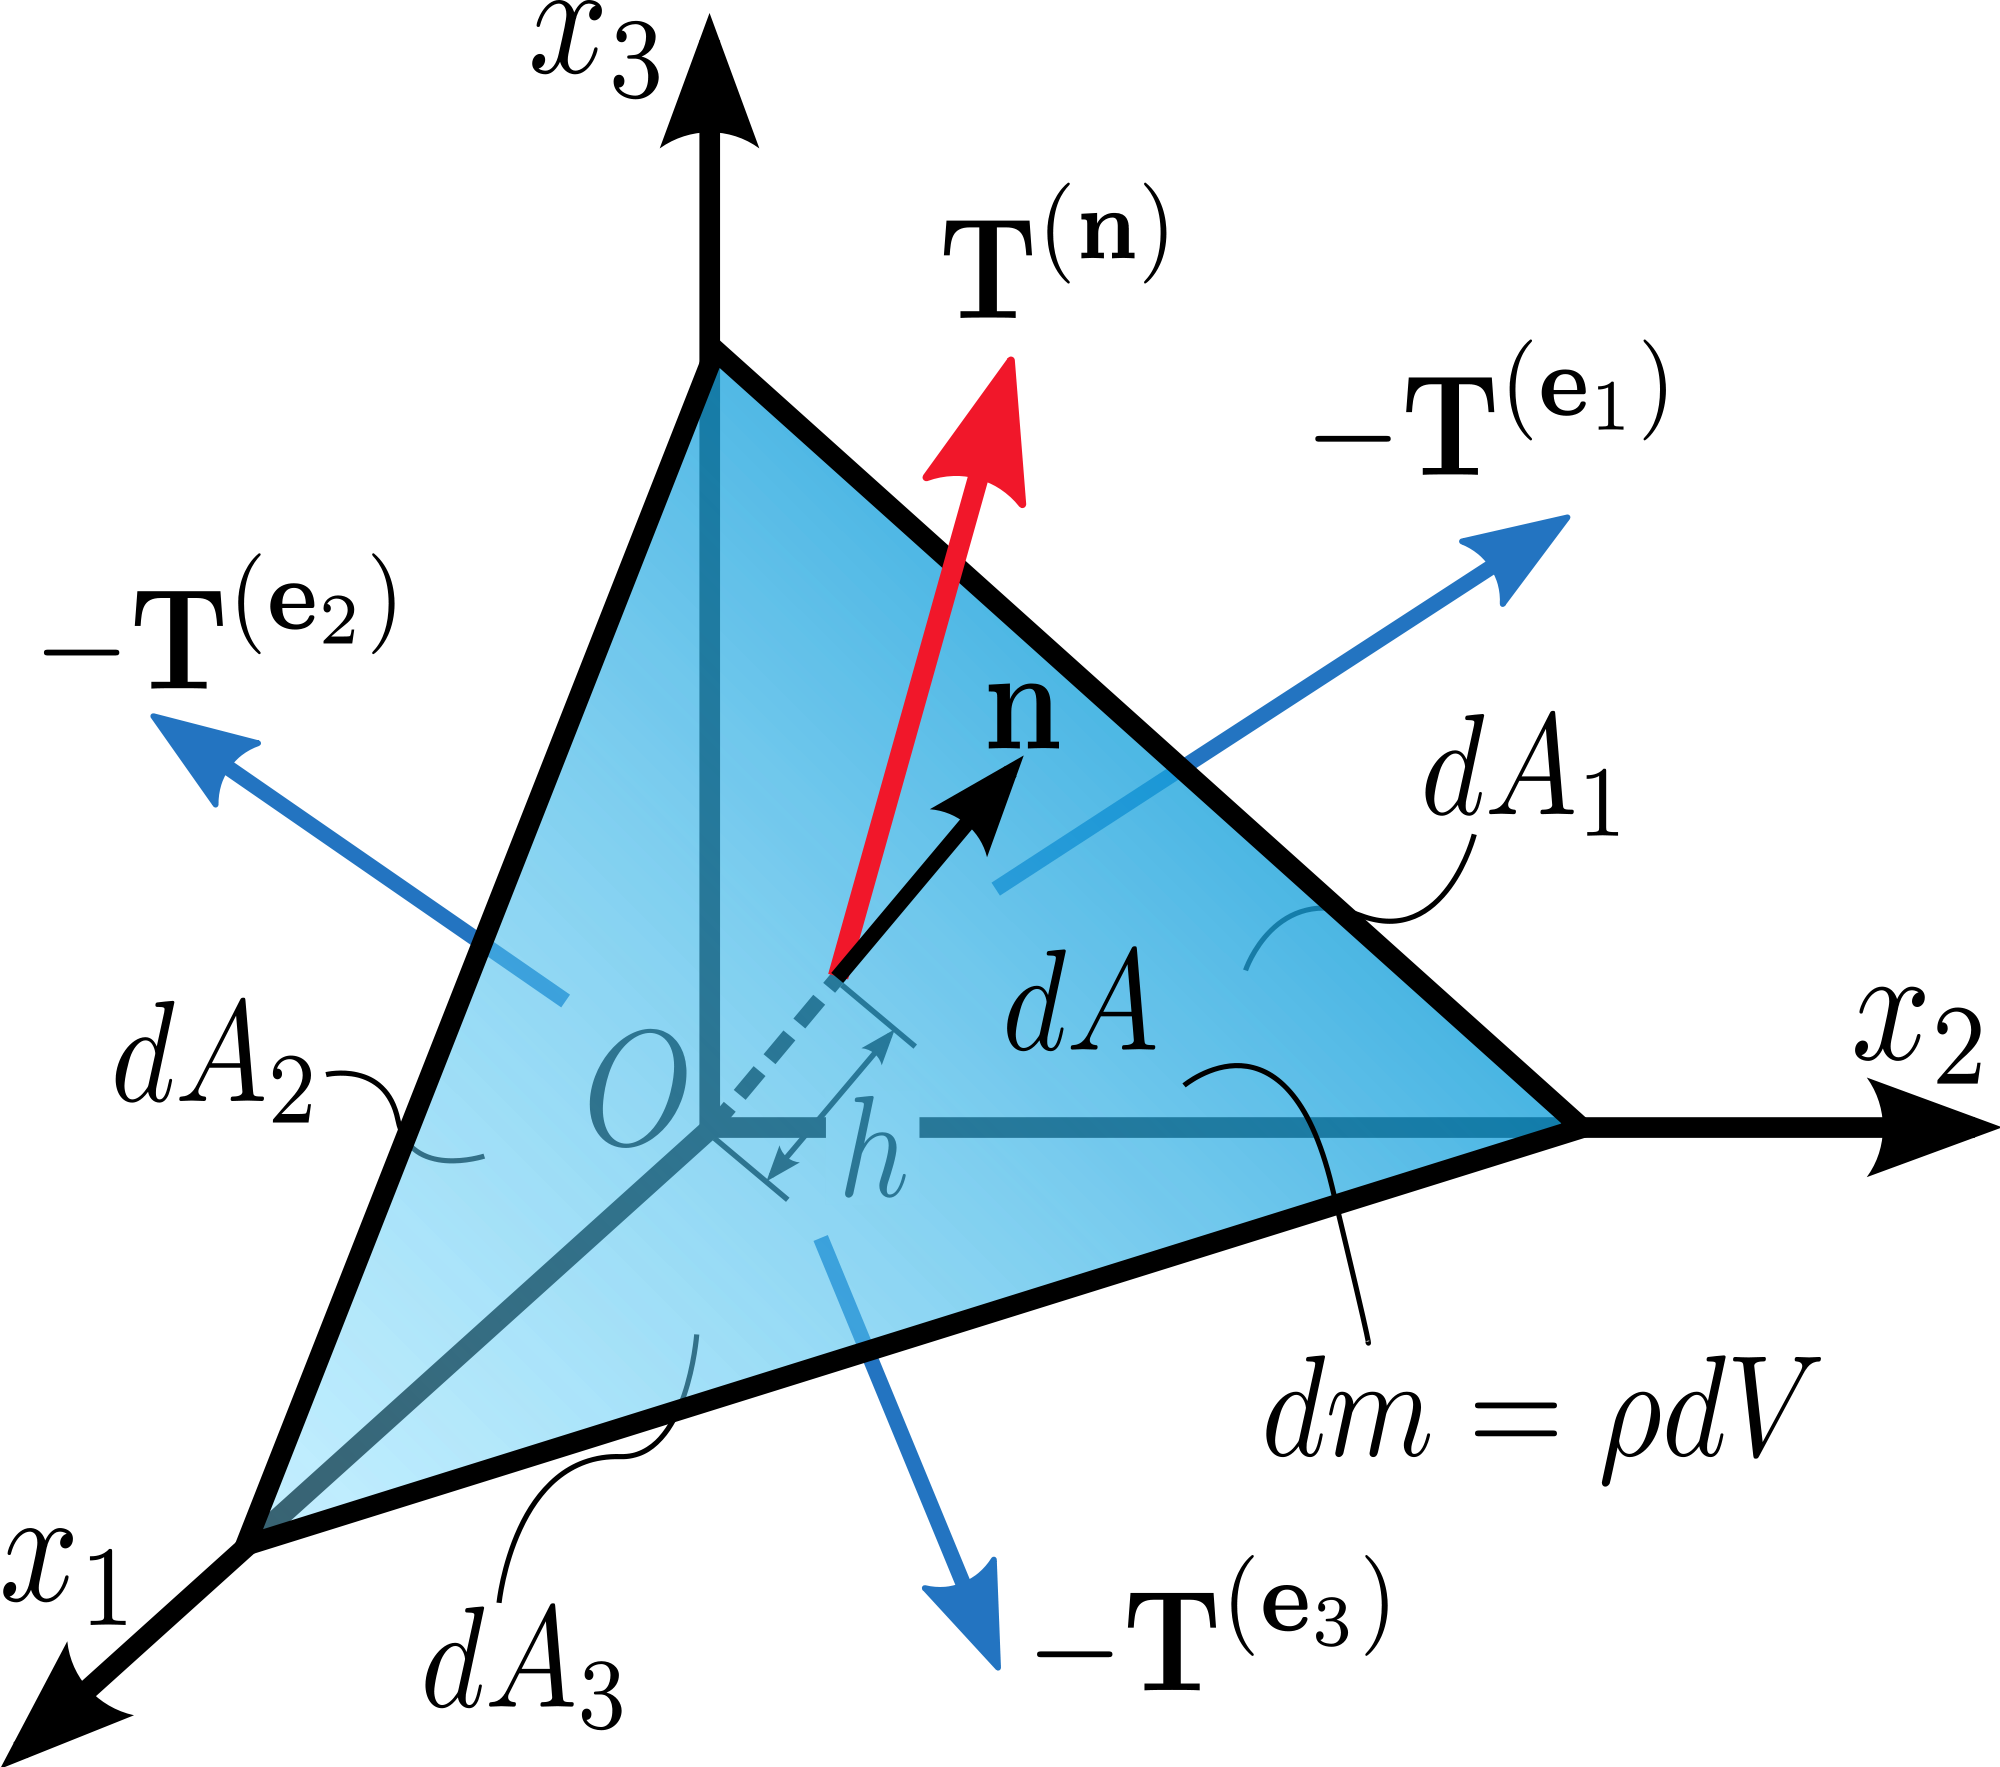
\includegraphics[width=\marginparwidth]{figs/intro/TetraCauchy}
\caption{Tetraedro de Cauchy}
\label{fig:TetraCauchy}
}
	
	\begin{equation}
		\begin{array}{c}
			\mathbf{T} = 
			\begin{bmatrix}
				T_1 ^{(\mathbf{n})} \\ T_2 ^{(\mathbf{n})} \\ T_3 ^{(\mathbf{n})}
			\end{bmatrix} = \begin{bmatrix}
			\sigma_x & \tau_{xy} & \tau_{xz} \\
			\tau_{yx} & \sigma_y & \tau_{yz} \\
			\tau_{zx} & \tau_{zy} & \sigma_z
		\end{bmatrix} \begin{bmatrix}
				n_1 \\ n_2 \\ n_3
			\end{bmatrix} \\ \\
			\boxed{\mathbf{T} = \bm{\sigma} \mathbf{n}}
		\end{array}
		\label{eq:tSigma}
	\end{equation}
	
	%%%%%%%%%%%%%%%%%%%%%%%
\subsection{Movimiento de un cuerpo}

\marginpar{
	\captionsetup{type=figure}
	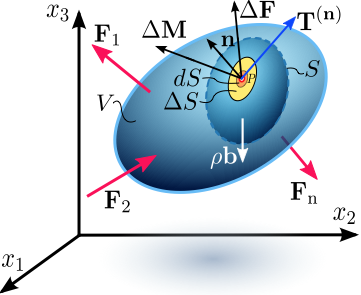
\includegraphics[width=\marginparwidth]{figs/intro/FuerzasCuerpo}
	\caption{Fuerzas sobre un cuerpo}
	\label{fig:FuerzasCuerpo}
\label{FuerzasCuerpo}
}
	
	Atendiendo la figura \ref{fig:FuerzasCuerpo} en donde se indican las fuerzas de superficie \index{fuerzas de superficie} 	$\mathbf{T}$ y las de cuerpo $\rho \mathbf{b}$, siendo $\rho$ la densidad del cuerpo en el punto $P$ y $\mathbf{b}$ la fuerza de cuerpo en $P$ por unidad de masa, puede escribirse las ecuaciones del movimiento, considerando la \textit{segunda Ley de Newton} sobre cada partícula que conforma el cuerpo y sumando en  todo el volumen, resulta así la siguiente
	ecuación\sidenote{Esta ecuación es además equivalente al teorema del impulso y la cantidad de movimiento lineal.}:
	
	\begin{equation}
		\int_S \mathbf{T} \, dS + \int_V \rho \mathbf{b} \, dV
		= \int_V \rho \mathbf{a} \, dV
	\end{equation}
	
	en la cual $\mathbf{a}$ es la aceleración de la partícula que ocupa el volumen $dV$.
	
	En la primera integral podemos sustituir $\mathbf{T}$
	por $\bm{\sigma} \mathbf{n}$ según lo visto en \eqref{eq:tSigma}
	
	\begin{equation}
		\int_S \bm{\sigma} \mathbf{n} \, dS + \int_V \rho \mathbf{b} \, dV
		= \int_V \rho \mathbf{a} \, dV
		\label{eq:parcial}
	\end{equation}
	
	Recordamos el \textit{teorema de Gauss}\index{teorema de Gauss} que posibilita substituir una integral de superficie por otra de volumen:
	
	\begin{equation}
		\int_S \bm{\sigma} \mathbf{n} \, dS = \int_V \nabla
		\bm{\sigma} \, dV
		\label{Gauss}
	\end{equation}
\marginnote[-.9cm]{\small Teorema de Gauss}

En donde: $\nabla = \begin{bmatrix}
	\dfrac{\partial}{\partial x} & \dfrac{\partial}{\partial y} & \dfrac{\partial}{\partial z}
\end{bmatrix}$ es el operador nabla.
	
	Usando \eqref{Gauss} en \eqref{eq:parcial} llegamos a
	\begin{equation}
		\int_V \left( \nabla \bm{\sigma}  + \rho \mathbf{b} - \rho
		\mathbf{a} \right) \, dV = \mathbf{0}
	\end{equation}
	
	como el volumen $V$ es arbitrario, se debe cumplir que:
	\begin{equation}
		\nabla \bm{\sigma} + \rho \mathbf{b} = \rho \mathbf{a}
		\label{mov1}
	\end{equation}
\marginnote[-.85cm]{\small Ecuación de movimiento}
	
	%%%%%%%%%%%%%%%%%%%
	\subsection{Ecuaciones de equilibrio}
	
	En el equilibrio, es decir, si el cuerpo está en reposo o con velocidad constante, la aceleración es nula $\mathbf{a} = \mathbf{0}$. Además si se llama $\mathbf{f} = \rho \mathbf{b}$ a la fuerza de cuerpo por unidad de volumen, entonces:
	
	\begin{equation}
		\boxed{\nabla \bm{\sigma} + \mathbf{f} = \mathbf{0}}
		\label{eq:equil}
	\end{equation}
	\marginnote[-.65cm]{\small Ecuación de equilibrio}
	
	Ya que el tensor de esfuerzos de Cauchy es simétrico, las \textit{ecuaciones de equilibrio} se pueden escribir, en su forma extendida:
	\begin{equation}
		\begin{array}{c}
			\dfrac{\partial \sigma_{x}}{\partial x} + \dfrac{\partial
				\tau_{xy}}{\partial y} + \dfrac{\partial \tau_{xz}}{\partial
				z} + f_x = 0 \\ \\
			\dfrac{\partial \tau_{xy}}{\partial y} + \dfrac{\partial
				\sigma_{y}}{\partial y} + \dfrac{\partial \tau_{yz}}{\partial
				z} + f_y = 0 \\ \\
			\dfrac{\partial \tau_{xz}}{\partial x} + \dfrac{\partial
				\tau_{yz}}{\partial y} + \dfrac{\partial \sigma_{z}}{\partial
				z} + f_z =0
		\end{array}
	\end{equation}
	
	Esta es la ``forma fuerte''\index{forma fuerte} de las ecuaciones diferenciales parciales de equilibrio.
	
\section{Deformación unitaria}
\index{Deformación unitaria}

\subsection{Desplazamiento}
\index{Desplazamiento}

Considere un punto material, de una estructura cualquiera, en la posición $\mathbf{r} = \begin{bmatrix}
	x & y & z
\end{bmatrix}^T $ de un sistema de coordenadas $xyz$ el cual se muestra en la fig. \ref{fig:desplaz}. Luego de la acción de las fuerzas el punto material sufre un desplazamiento $\mathbf{u} = \begin{bmatrix}
u & v & w
\end{bmatrix}^T$ y se ubica en $\mathbf{s} = \begin{bmatrix}
x + u & y + v & z + w
\end{bmatrix}^T$.

\begin{figure}[ht]
	\centering
	\begin{tikzpicture}[scale=1]
		\draw[-latex] (-1, 0, 0) -- (5, 0, 0) node[below left]{$x$};
		\draw[-latex] (0, -1, 0) -- (0, 5, 0) node[left]{$y$};
		\draw[-latex] (0, 0, -1) -- (0, 0, 5) node[left]{$z$};
		
		\coordinate (o) at (0, 0, 0);
		\coordinate (r) at (2, 3, 1);
		\coordinate (u) at (2, -1, 0);
		\coordinate (s) at ($(r)+(u)$);
		\coordinate (dr) at (-1, 1, -1);
		\coordinate (rdr) at ($(r) + (dr)$);
		
		\draw[thick, -latex, red] (o) -- (r) node[left, pos=.7]{$\mathbf{r}$};
		\draw[thick, -latex, blue] (r) -- (s) node[below, pos=.47]{$\mathbf{u}(\mathbf{r})$};
		\draw[thick, -latex, red] (o) -- (s) node[above, pos=.5]{$\mathbf{s}$};
		\draw[thick, -latex, red] (o) -- (rdr) node[above, pos=.7, rotate=76]{$\mathbf{r} + \Delta \mathbf{r}$};
		\draw[thick, -latex, blue] (r) -- (rdr) node[left, pos=.25]{$\Delta \mathbf{r}$};
		\draw[thick, -latex, red] (o) -- ($(s)+(dr)$) node[above, rotate=47, pos=.6]{$\mathbf{r} + \Delta \mathbf{s}$};
		\draw[thick, -latex, blue] (s) -- ($(s)+(dr)$) node[right, pos=.5]{$\Delta \mathbf{s}$};
		\draw[thick, -latex, blue] (rdr) -- ($(rdr)+(u)$) node[above, pos=.5, rotate=-27]{$\Delta \mathbf{u}(\mathbf{r} + \Delta \mathbf{r})$};
	\end{tikzpicture}
\caption{Desplazamiento}
\label{fig:desplaz}
\end{figure}

Ahora considere una partícula vecina en la posición $\mathbf{r} + \Delta \mathbf{r}$. En la configuración desplazada, la nueva posición de este punto será:
\begin{equation}
	\mathbf{s} + \Delta \mathbf{s} = \mathbf{r} + \Delta \mathbf{r} + \mathbf{u}(\mathbf{r} + \Delta \mathbf{r})
\end{equation}

por lo tanto (ver fig. \ref{fig:desplaz}):
\begin{equation}
	\Delta \mathbf{s} = \Delta \mathbf{r} + \mathbf{u}(\mathbf{r} + \Delta \mathbf{r}) - \mathbf{u}(\mathbf{r})
	\label{eq:ese}
\end{equation}
	
Si $\Delta \mathbf{u} = \mathbf{u}(\mathbf{r} + \Delta \mathbf{r}) - \mathbf{u}(\mathbf{r})$ es suficientemente pequeño:
\begin{equation}
	\begin{split}
	\Delta\mathbf{u} = \begin{bmatrix}
		\Delta u \\ \Delta v \\ \Delta w
	\end{bmatrix} & \approx \begin{bmatrix}
		\dfrac{\partial u}{\partial x} \Delta x + \dfrac{\partial u}{\partial y} \Delta y + \dfrac{\partial u}{\partial z} \Delta z \\[5mm]
		\dfrac{\partial v}{\partial x} \Delta x + \dfrac{\partial v}{\partial y} \Delta y + \dfrac{\partial v}{\partial z} \Delta z \\[5mm]
		\dfrac{\partial w}{\partial x} \Delta x + \dfrac{\partial w}{\partial y} \Delta y + \dfrac{\partial w}{\partial z} \Delta z
	\end{bmatrix} = \begin{bmatrix}
	\dfrac{\partial u}{\partial x} & \dfrac{\partial u}{\partial y} & \dfrac{\partial u}{\partial z} \\[5mm]
	\dfrac{\partial v}{\partial x} & \dfrac{\partial v}{\partial y} & \dfrac{\partial v}{\partial z} \\[5mm]
	\dfrac{\partial w}{\partial x} & \dfrac{\partial w}{\partial y} & \dfrac{\partial w}{\partial z}
\end{bmatrix} \begin{bmatrix}
\Delta x \\ \Delta y \\ \Delta z
\end{bmatrix} \\[5mm] &= \bm{\alpha} \Delta \mathbf{r}
\end{split}
\label{eq:Delta_u}
\end{equation}

En donde:
\begin{equation}
	\bm{\alpha} \coloneqq \begin{bmatrix}
		\dfrac{\partial u}{\partial x} & \dfrac{\partial u}{\partial y} & \dfrac{\partial u}{\partial z} \\[5mm]
		\dfrac{\partial v}{\partial x} & \dfrac{\partial v}{\partial y} & \dfrac{\partial v}{\partial z} \\[5mm]
		\dfrac{\partial w}{\partial x} & \dfrac{\partial w}{\partial y} & \dfrac{\partial w}{\partial z}
	\end{bmatrix} = \left( \nabla \mathbf{u}^T \right)^T
\end{equation}

Se observa de \eqref{eq:ese} y \eqref{eq:Delta_u} que:

\begin{equation}
	\Delta \mathbf{s} = \left( \mathbf{I} + \bm{\alpha} \right) \Delta \mathbf{r}
	\label{eq:Delta_s}
\end{equation}

\subsection{Tensor deformación unitaria}
\index{Tensor deformación unitaria}
A continuación se calcula la norma del vector $\Delta \mathbf{s}$ dado por \eqref{eq:Delta_s}, que en un entorno infinitesimal será:

\begin{equation}
	|| d \mathbf{s} ||^2 = \left(d \mathbf{s}\right)^T d \mathbf{s} = \left(d \mathbf{r}\right)^T \left( \mathbf{I} + \bm{\alpha}^T \right) \left( \mathbf{I} + \bm{\alpha} \right) d \mathbf{r} = \left(d \mathbf{r}\right)^T \left(\mathbf{I} + 2 \mathbf{E} \right) d \mathbf{r}
\end{equation}

En donde:
\begin{equation}
	\mathbf{E} = \dfrac{1}{2} \left(\bm{\alpha} + \bm{\alpha}^T + \bm{\alpha}\bm{\alpha}^T \right)
\end{equation}
\marginnote[-1cm]{\small Tensor deformación unitaria de Green - Saint-Venant}

Notar que $\mathbf{E}$ es un tensor simétrico.

Despreciando en $\mathbf{E}$, el término de segundo orden, se obtiene el tensor (simétrico) deformación unitaria que se define como:

\begin{equation}
	\begin{split}
		\bm{\varepsilon} & \coloneqq \dfrac{1}{2} \left(\bm{\alpha} + \bm{\alpha}^T \right) \\ &=  \begin{bmatrix}
		\dfrac{\partial u}{\partial x} & \dfrac{1}{2} \left(\dfrac{\partial u}{\partial y} + \dfrac{\partial v}{\partial x}\right) & \dfrac{1}{2} \left(\dfrac{\partial u}{\partial z} + \dfrac{\partial w}{\partial x}\right) \\[5mm]
		\dfrac{1}{2} \left(\dfrac{\partial v}{\partial x} + \dfrac{\partial u}{\partial y}\right) & \dfrac{\partial v}{\partial y} & \dfrac{1}{2} \left(\dfrac{\partial v}{\partial z} + \dfrac{\partial w}{\partial y}\right) \\[5mm]
		\dfrac{1}{2} \left(\dfrac{\partial w}{\partial x} + \dfrac{\partial u}{\partial z}\right) & \dfrac{1}{2} \left(\dfrac{\partial w}{\partial y} + \dfrac{\partial v}{\partial z}\right) & \dfrac{\partial w}{\partial z}
	\end{bmatrix}
	\end{split}
\end{equation}

de donde:
\begin{equation}
	\bm{\varepsilon} = \begin{bmatrix}
		\varepsilon_{11} & \varepsilon_{12} & \varepsilon_{13} \\
		\varepsilon_{21} & \varepsilon_{22} & \varepsilon_{23} \\
		\varepsilon_{31} & \varepsilon_{32} & \varepsilon_{33}
	\end{bmatrix} = \begin{bmatrix}
		\varepsilon_x & \dfrac{1}{2} \gamma_{xy} & \dfrac{1}{2} \gamma_{xz} \\[5mm]
		\dfrac{1}{2} \gamma_{yx} & \varepsilon_y & \dfrac{1}{2} \gamma_{yz} \\[5mm]
		\varepsilon_x & \dfrac{1}{2} \gamma_{xy} & \varepsilon_z \\
	\end{bmatrix}
\end{equation}

Es fácil ver que este tensor es simétrico, por lo que $\gamma_{ij} = \gamma_{ji}$. Debido a este hecho se puede definir el \textit{vector deformación unitaria}:

\begin{equation}
	\underline{\bm{\varepsilon}} \coloneqq \begin{bmatrix}
		\varepsilon_x & \varepsilon_y & \varepsilon_z & \gamma_{yz} & \gamma_{xz} & \gamma_{xy}
	\end{bmatrix}^T
\end{equation}

\section{Relaciones constitutivas}

Se supone un material elástico lineal, homogéneo e isotrópico. En este caso son necesarias dos constantes para relacionar linealmente las tensiones con las deformaciones unitarias.

\subsection{Constantes de Lamé}
\index{Constantes de Lamé}
La propuesta de relación lineal que define las constantes de Lamé\sidenote{Gabriel Lamé, francés (22 Julio 1795 – 1 Mayo 1870)} $\mu$ y $\lambda$, es:

\begin{equation}
	\bm{\sigma} = 2 \mu \bm{\varepsilon} + \lambda \mathsf{tr} \left( \bm{\varepsilon} \right) \mathbf{I}
\end{equation}

\subsection{Ley de Hooke}
\index{Ley de Hooke}
En ingeniería es más usual, utilizar la ley de Hooke\sidenote{Robert Hooke, inglés (18 Julio 1635 – 3 Marzo 1703)}, con las constantes $E$ y $\nu$, que son respectivamente el módulo de elasticidad o de Young\sidenote{Thomas Young, inglés (13 Junio 1773 – 10 Mayo 1829)} y el módulo de Poisson\sidenote{Siméon Denis Poisson, francés (21 Junio 1781 – 25 Abril 1840)}.

\begin{equation}
	\begin{split}
		\varepsilon_x &= \dfrac{\sigma_x}{E} - \nu \dfrac{\sigma_y}{E} - \nu \dfrac{\sigma_z}{E}\\[5mm]
		\varepsilon_x &= -\nu \dfrac{\sigma_x}{E} + \dfrac{\sigma_y}{E} - \nu \dfrac{\sigma_z}{E}\\[5mm]
		\varepsilon_x &= -\nu \dfrac{\sigma_x}{E} - \nu \dfrac{\sigma_y}{E} + \dfrac{\sigma_z}{E}\\[5mm]
		\gamma_{yz} &= \dfrac{\tau_{yz}}{G}; \quad \gamma_{xz} = \dfrac{\tau_{xz}}{G} \quad
		\gamma_{xy} = \dfrac{\tau_{xy}}{G}
	\end{split}
\end{equation}

En donde, el módulo de corte $G = \dfrac{E}{2 (1 + \nu)}$

Con los vectores $\bm{\sigma}$ y $\bm{\varepsilon}$, la relación anterior, matricialmente, se puede escribir:

\begin{equation}
	\underline{\bm{\sigma}} = \mathbf{D} \underline{\bm{\varepsilon}}
\end{equation}

En donde, $\mathbf{D}$ es una matriz simétrica $6 \times 6$.

\begin{equation}
	\mathbf{D} = \dfrac{E}{(1+\nu)(1-2\nu)}
	\begin{bmatrix}
		1-\nu & \nu & \nu & 0 & 0 & 0 \\
		\nu & 1-\nu & \nu & 0 & 0 & 0 \\
		\nu & \nu & 1-\nu & 0 & 0 & 0 \\
		0 & 0 & 0 & 0.5-2\nu & 0 & 0 \\
		0 & 0 & 0 & 0 & 0.5-2\nu & 0 \\
		0 & 0 & 0 & 0 & 0 & 0.5-2\nu
	\end{bmatrix}
\end{equation}


\subsection{Energía potencial total}

La energía potencial total\index{energía potencial total} del sistema estructural se define como:

\begin{equation}
	\Pi = U + W
	\label{eq:EP}
\end{equation}

Siendo $U$ la energía de deformación unitaria\index{energía de deformación unitaria} y $W$ el potencial de trabajo\index{potencial de trabajo}. La energía de deformación unitaria es:

\begin{equation}
	U = \dfrac{1}{2} \int_V \underline{\bm{\sigma}}^T \underline{\bm{\varepsilon}} \, dV
\end{equation}

El potencial de trabajo está dado por:

\begin{equation}
	W = -\int_V \mathbf{u}^T \mathbf{f} \, dV - \int_S \mathbf{u}^T \mathbf{T} \, dS - \sum_i \mathbf{u}^T_i \mathbf{P}_i
\end{equation}


\index{Principio de mínima energía potencial}

\begin{kaobox}[frametitle=Principio de mínima energía potencial]
	Para sistemas conservativos, de todos los campos de desplazamientos cinemáticamente admisibles, aquellos que corresponden a condiciones de equilibrio, extremizan la energía potencial total. Si la condición extrema es un mínimo, el estado de equilibrio es estable
\end{kaobox}

\section{Energía y ecuaciones de campo de elementos estructurales}

\subsection{Barra con carga axial}

En la fig. \ref{fig:barra-carga-axial} se muestra una barra de sección variable con carga axial, su ecuación diferencial gobernante es:
\begin{equation}
	\dfrac{d}{dx} \left( AE \dfrac{du}{dx} \right) + p = 0
	\label{eq:barra-axial}
\end{equation}

\marginpar{
	\captionsetup{type=figure}
	\includestandalone[width=\marginparwidth]{figs/fundamentales/barra-carga-axial}
	\caption{Barra con carga axial}
	\label{fig:barra-carga-axial}
}

Si $AE = cte.$ \eqref{eq:barra-axial} se convierte en:
\begin{equation}
	AE \dfrac{d^2u}{dx^2} + p = 0
\end{equation}

Por otro lado, la energía potencial total es:

\begin{equation}
	\Pi = \dfrac{1}{2} \int_L \sigma \varepsilon A \, dx - \int_L up\, dx - \sum_i u_i P_i
	\label{eq:energia_unidimensionales}
\end{equation}

como $\sigma A = EA \varepsilon = EA \dfrac{du}{dx}$, entonces:

\begin{equation}
	\Pi = \dfrac{1}{2} \int_L EA \left( \dfrac{du}{dx} \right)^2 \, dx - \int_L up\, dx - \sum_i u_i P_i
	\label{eq:eptuni}
\end{equation}

\subsection{Vigas}

La fig. \ref{fig:viga} muestra un caso particular de viga, en general la ecuación diferencial gobernante es:

\begin{equation}
	\dfrac{d^2}{dx^2} \left( EI \dfrac{d^2v}{dx^2}\right) - q = 0
	\label{eq:ed-viga}
\end{equation}

\marginpar{
	\captionsetup{type=figure}
	\includestandalone[width=\marginparwidth]{figs/fundamentales/viga0}
	\caption{Viga con carga distribuida.}
	\label{fig:viga}
}

Si $EI = cte.$ \eqref{eq:ed-viga} se convierte en:

\begin{equation}
	\dfrac{d^4v}{dx^4} - \dfrac{q}{EI} = 0
	\label{eq:ed-viga-cte}
\end{equation}

La energía potencial total es:
\begin{equation}
	\Pi = \frac{1}{2} \int_L EI \left(\frac{d^2v}{dx^2}\right)^2 \, dx - \int_L vq \, dx - \sum_i v_iP_i
	\label{eq:energia-vigas}
\end{equation}

en donde $v = v(x)$ es el campo de desplazamientos verticales de la viga, con carga 
distribuida $q = q(x)$ y puntuales $P_i$ (las cargas se consideran positivas hacia 
arriba, coherentes con el sentido positivo de $v$).

\subsection{Losas}

En la fig. \ref{fig:losa0}, se representa una losa cargada. La ecuación diferencial gobernante es \cite{timoshenko1959theory}:
\begin{equation}
	 \dfrac{\partial^4 w}{\partial x^4} + 2\dfrac{\partial^4 w}{\partial x^2y^2} + \dfrac{\partial^4 w}{\partial y^4} - \dfrac{q}{D} = 0
\end{equation}
\marginpar{
	\captionsetup{type=figure}
	\includestandalone[width=\marginparwidth]{figs/fundamentales/losa0}
	\caption{Losa cargada.}
	\label{fig:losa0}
}
con:
\begin{equation}
	D = \dfrac{Eh^3}{12 (1 - \nu^2)}
\end{equation}

O también:
\begin{equation}
	\laplace^2 w - \dfrac{q}{D} = 0
\end{equation}

en donde $\laplace (\cdot)$ es el operador de Laplace:
\begin{equation}
	\laplace (\cdot) = \nabla^2 (\cdot) = \dfrac{\partial^2 (\cdot)}{\partial x^2} + \dfrac{\partial^2 (\cdot)}{\partial y^2}
\end{equation}

La energía de deformación unitaria es:
\begin{equation}
	U = \frac{1}{2} \iint_S D \left[ \left( \frac{\partial^2 w}{\partial x^2} \right)^2 + 2 \frac{\partial^2 w}{\partial x^2} \frac{\partial^2 w}{\partial y^2} + \left( \frac{\partial^2 w}{\partial x^2} \right)^2 \right] \ dx dy
\end{equation}

Por lo tanto, la energía potencial total es:

\begin{equation}
	\Pi = \frac{1}{2} \iint_S D \left( \laplace^2 w \right)^2 \ dx dy - \iint_S w q \ dx dy
\end{equation}
